% Author: Max Melching, 2025
% With elements from https://tikz.net/hyperbola/
\documentclass[border=3pt,tikz]{standalone}


\usepackage{tikz}
\usepackage{pgfplots} % for the axis environment
\usepackage[outline]{contour}
\usepackage{xcolor}
\usepackage{newtxmath}  % Use Times in math mode
\usepackage{tgpagella}  % Use Pagella in text


\colorlet{mydarkred}{red!70!black}
\colorlet{mydarkgreen}{green!50!black}


\usetikzlibrary{arrows.meta, calc, decorations.markings, through, intersections}


\tikzset{
    >={Stealth[inset=0,angle'=27]},
    lab velocity/.style={
        ->,
        thick,
    },
    com velocity/.style={
        ->,
        thick,
        mydarkgreen,
    },
    angle/.style={
        ->,
        semithick,
        % scale=0.5,  % Trying to make arrow tip smaller
        mydarkred,
    },
}



\begin{document}


% V < v'_1
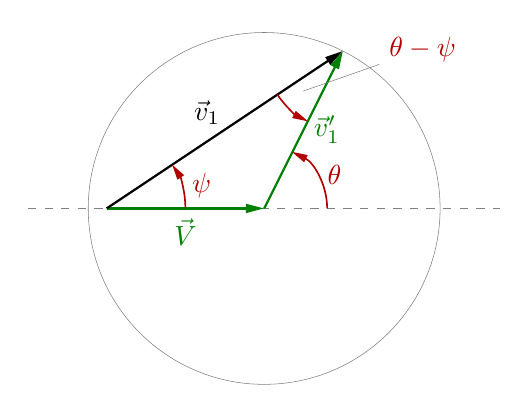
\begin{tikzpicture}
    \coordinate (O) at (0, 0);
    \coordinate (V) at (2, 0);
    \coordinate (v1) at (3, 2);


    % \draw[dashed, gray] (V) --++ (V);
    \draw[help lines, dashed] ($-0.5*(V)$) -- ($2.5*(V)$);

    \draw[com velocity] (O) -- (V) node[midway, below] {$\vec{V}$};
    \draw[lab velocity] (O) -- (v1) node[midway, above left=-2] {$\vec{v}_1$};
    \draw[com velocity] (V) -- (v1) node[midway, right] {$\vec{v}'_1$};


    % \pgfmathsetmacro{\r}{sqrt((2-3)^2 + (0-2)^2)}
    % \draw (V) circle(\r);

    \node[draw, help lines] at (V) [circle through={(v1)}] {};


    \def\arcrad{0.8}
    \def\rtheta{64}
    \draw[angle] (V) ++ (\arcrad,0) arc(0:\rtheta:\arcrad) node[midway, right] {$\theta$};
    \def\arcrad{1}
    \def\rpsi{34}
    \draw[angle] (O) ++ (\arcrad,0) arc(0:\rpsi:\arcrad) node[midway, right] {$\psi$};
    % \draw[angle] ($(V) + (\arcrad,0)$) arc(0:\rtheta:\arcrad) node[midway, right] {$\theta$};
    % \draw[angle] ($(O) + (\arcrad,0)$) arc(0:\rpsi:\arcrad) node[midway, right] {$\psi$};

    \pgfmathsetmacro{\vonenorm}{sqrt((3)^2 + (2)^2)}
    \draw[angle, rotate=\rpsi] (v1) ++ ($-\arcrad/\vonenorm*(v1)$) arc(0:\rtheta-\rpsi:-\arcrad);

    % \coordinate (labelpos) at ($0.1*(V) + 0.8*(v1)$);
    \coordinate (labelpos) at ($(v1) - \arcrad/\vonenorm*(v1) + 0.1*(V)$);

    \begin{scope}[angle, -, pin distance=1cm]
        \node[pin=15:$\theta - \psi$] at (labelpos) {};
    \end{scope}
\end{tikzpicture}



% V > v'_1
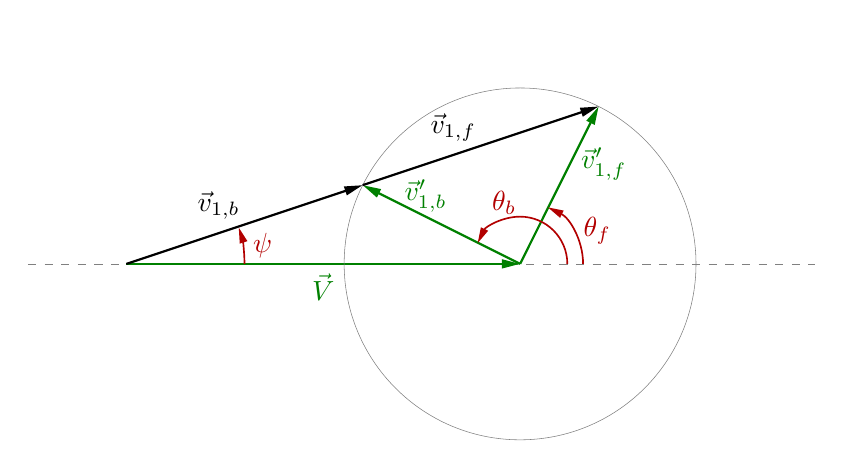
\begin{tikzpicture}
    \coordinate (O) at (0, 0);
    \coordinate (V) at (5, 0);
    \coordinate (v1) at (3, 1);


    % \draw[dashed, gray] (V) --++ (V);
    \draw[help lines, dashed] ($-0.25*(V)$) -- ($1.75*(V)$);
    \draw[com velocity] (O) -- (V) node[midway, below] {$\vec{V}$};

    \node[draw, help lines, name path=circle] at (V) [circle through={(v1)}] {};
    \path[name path=vel1] (O) -- ($3*(v1)$);
    \path[name intersections={of=circle and vel1,by={v1f,v1b}}];  % Order determined by testing
    \draw[lab velocity] (O) -- (v1b) node[pos=0.5, above left=-2] {$\vec{v}_{1, b}$};
    \draw[com velocity] (V) -- (v1b) node[pos=0.6, above=-2] {$\vec{v}'_{1, b}$};
    \draw[lab velocity] (v1b) -- (v1f) node[pos=0.5, above left=-2] {$\vec{v}_{1, f}$};
    \draw[com velocity] (V) -- (v1f) node[pos=0.75, below right=-3] {$\vec{v}'_{1, f}$};


    \def\arcrad{0.8}
    \def\rtheta{64}
    \draw[angle] (V) ++ (\arcrad,0) arc(0:\rtheta:\arcrad) node[midway, right] {$\theta_f$};
    \def\arcrad{0.6}
    \draw[angle] (V) ++ (\arcrad,0) arc(0:\rtheta+90:\arcrad) node[pos=0.6, above left=-3] {$\theta_b$};
    \def\arcrad{1.5}
    \def\rpsi{18}
    \draw[angle] (O) ++ (\arcrad,0) arc(0:\rpsi:\arcrad) node[midway, right] {$\psi$};
\end{tikzpicture}


\end{document}